% ========================================
% CAPÍTULO 1: INTRODUCCIÓN Y FORMULACIÓN DEL PROBLEMA  (criterio 1 de la rúbrica)
% ========================================

\chapter{INTRODUCCIÓN Y FORMULACIÓN DEL PROBLEMA}
\label{ch:introduccion}

\section{Contexto}

Los asistentes de programación basados en modelos de lenguaje grande (LLM) ya escriben pipelines completos de ciencia de datos \parencite{hong2025} y se evalúan con \emph{benchmarks} de generación de código \parencite{lai2023}, y los \emph{benchmarks} de agentes miden su puntaje o su tasa de éxito \parencite{chan2025,huang2024}, no la validez metodológica de lo que producen. Un código generado por un LLM puede fallar de siete formas habituales: (1) errores de sintaxis; (2) alucinación de APIs o uso de métodos obsoletos; (3) incompatibilidad de dimensiones o tipos; (4) ineficiencia o agotamiento de memoria; (5) falta de control de semillas; (6) manejo inseguro de archivos o credenciales; y (7) \textbf{fuga de datos} (\emph{data leakage}).

La fuga es el único de los siete que \textbf{no interrumpe la ejecución}. Los fallos 1 a 4 y 6 producen una excepción o son visibles para un \emph{linter}, y el fallo 5 se detecta repitiendo la corrida. En cambio, la fuga produce un script que corre de principio a fin, entrega métricas más altas y, por eso, rara vez se cuestiona (Tabla~\ref{tab:ruidoso}). En la práctica humana el problema es amplio: \textcite{kapoor2023} hallaron 294 artículos afectados por fuga en 17 campos científicos, y \textcite{kaufman2012} la formularon como información del objetivo que no estaría disponible al predecir.

\begin{table}[H]
\centering
\caption{Fallos ruidosos frente a fallo silencioso en código de ML generado por LLM.}
\label{tab:ruidoso}
\begingroup\footnotesize\singlespacing
\begin{tabular}{@{}p{3.4cm} p{4.6cm} p{7.4cm}@{}}
\toprule
Dimensión & Fallos ruidosos (1--4 y 6) & Fuga de datos (7) \\
\midrule
Comportamiento del intérprete & Lanza una excepción & Se ejecuta sin error ni advertencia \\
Detección estándar & Intérprete o \emph{linter} & Invisible para herramientas convencionales: tipos y dimensiones coinciden \\
Efecto sobre las métricas & No llega a producirlas & Las infla (optimismo) \\
Riesgo en producción & Bajo: el pipeline no corre & Alto: el modelo se despliega con una capacidad de generalización peor que la creída \\
\bottomrule
\end{tabular}
\endgroup
\end{table}

\section{Qué es la fuga y cómo ocurre en scikit-learn}

Un transformador (escalador, imputador, selector de variables, PCA) \emph{aprende} parámetros con \texttt{.fit()}: medias y desviaciones, vecinos más cercanos, o qué variables conservar. Si aprende con \textbf{todas} las filas antes de separar entrenamiento y prueba, o fuera de un \texttt{Pipeline} dentro de una validación cruzada, ya vio las filas que luego se usan para evaluar. Formalmente, el aislamiento correcto exige que los parámetros del preprocesamiento sean función solo de los datos de entrenamiento; hay fuga cuando algún parámetro se estima con la unión de entrenamiento y prueba. La Figura~\ref{fig:codigo} contrasta ambas formas con el mismo modelo, los mismos datos y los mismos pliegues.

\begin{figure}[H]
\centering
\begin{footnotesize}
\begin{verbatim}
# CON FUGA: el escalador ve todas las filas
X_esc = StandardScaler().fit_transform(X)
scores = cross_val_score(modelo, X_esc, y, cv=5)

# SIN FUGA: en cada pliegue, .fit() ve solo el entrenamiento
pipe = Pipeline([("escalador", StandardScaler()), ("modelo", modelo)])
scores = cross_val_score(pipe, X, y, cv=5)
\end{verbatim}
\end{footnotesize}
\caption{Misma operación con y sin fuga de datos.}
\label{fig:codigo}
\end{figure}

Para ver el mecanismo con números, el script \arch{demo_fuga.py} ejecuta ambas formas con \texttt{breast\_cancer}, un \texttt{KNNImputer}, un escalador, \texttt{SelectKBest} y una red \texttt{MLPClassifier}, con los mismos pliegues (Figura~\ref{fig:demo}). Con datos reales, el ROC-AUC es 0,979 con fuga y 0,977 sin ella: $\DOpt=+0{,}0015$, casi invisible porque la señal es muy fuerte. Con 500 columnas de ruido y etiquetas permutadas (verdad: AUC $=0{,}5$), sube a 0,571 frente a 0,523 ($\DOpt=+0{,}048$): el selector «encuentra» columnas que por azar parecen predecir.

\begin{figure}[H]
\centering
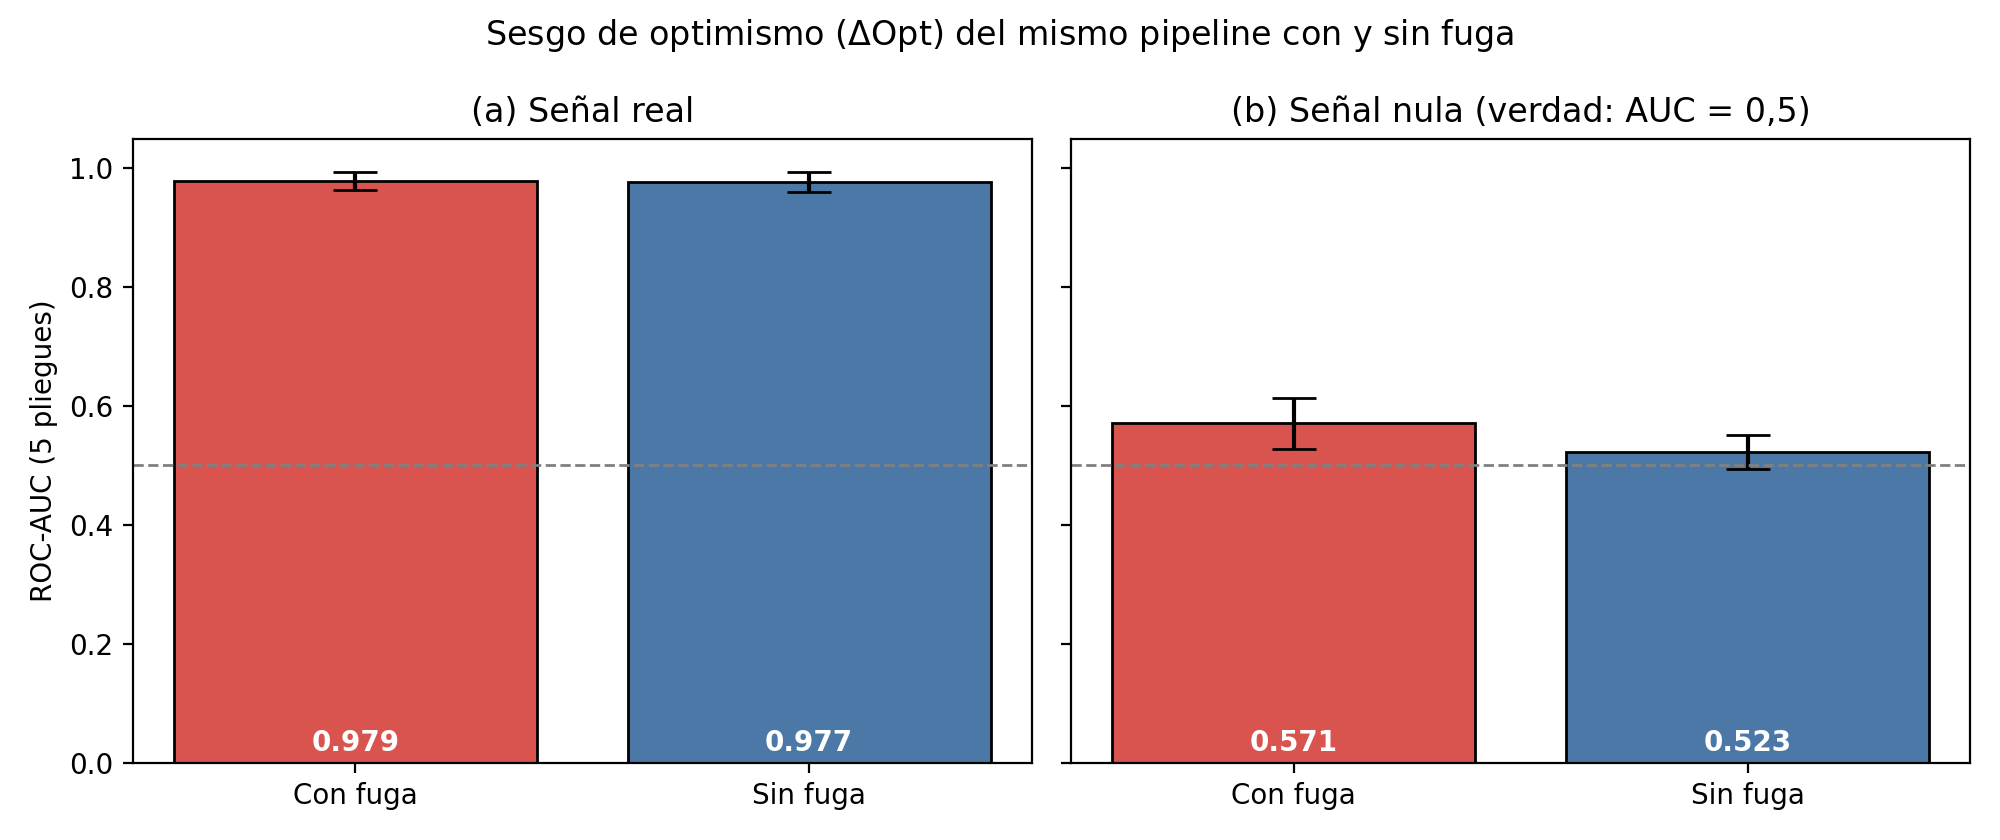
\includegraphics[width=0.85\textwidth]{fig_demo_fuga.png}
\caption{Mismo pipeline con y sin fuga. (a) Señal real. (b) Señal nula; la línea punteada marca el AUC verdadero (0,5).}
\label{fig:demo}
\end{figure}

Se estudian cuatro mecanismos: \textbf{escalado} (la media y la varianza incluyen filas de prueba), \textbf{imputación} (\texttt{KNNImputer} puede copiar valores de vecinos de prueba), \textbf{selección de variables} (\texttt{SelectKBest} usa las etiquetas de todas las filas) y \textbf{combinada} (los tres a la vez).

\section{Problema, pregunta y relevancia}

\textbf{Problema.} Un script de ML tabular puede contener fuga de datos sin que nada lo advierta, y quien recibe ese código de un asistente de IA no tiene una forma barata de comprobarlo ni de saber cuánto distorsiona la evaluación.

\textbf{Pregunta de investigación.} ¿Es posible detectar automáticamente, leyendo y ejecutando el código, la fuga de preprocesamiento y selección en pipelines de scikit-learn; reparar el código sin cambiar el modelo; y cuantificar cuánto optimismo introduce la fuga en distintas familias de algoritmos?

\textbf{Relevancia.} Los detectores existentes son principalmente estáticos y se evaluaron sobre código humano \parencite{yang2022,drobnjakovic2024,alomar2025}, y los LLM tienen dificultades para identificar por sí mismos estos problemas tempranos del pipeline \parencite{kumar2025}. Falta un instrumento determinista que audite código de asistentes, lo repare y mida el daño; ese es el entregable de este proyecto.

\section{Objetivos}

\textbf{Objetivo general.} Diseñar, validar empíricamente e implementar un marco automatizado de detección y prevención de fuga de datos en pipelines de aprendizaje supervisado con scikit-learn, y cuantificar el sesgo de optimismo que induce en cuatro familias de algoritmos.

\begin{table}[H]
\centering
\caption{Objetivos específicos verificables y evidencia.}
\label{tab:oe}
\begingroup\footnotesize\singlespacing
\begin{tabular}{@{}l p{9.4cm} p{4.4cm}@{}}
\toprule
OE & Objetivo específico & Evidencia \\
\midrule
OE1 & Formalizar los mecanismos de fuga (escalado, imputación, selección, combinada) y distinguirlos de otros fallos de código generado. & Secciones 1.1--1.2; banco de 96 pares \\
OE2 & Desarrollar un auditor determinista (AST y verificación en ejecución) y medir su precisión, recall y VPN contra una verdad conocida. & Tablas~\ref{tab:banco} y \ref{tab:indep} \\
OE3 & Cuantificar el Sesgo de Optimismo \DOpt{} por tipo de fuga y familia (RandomForest, Gradient Boosting, lineal regularizado y red neuronal MLP) en 3 datasets de clasificación y 3 de regresión. & Tablas~\ref{tab:dopt} y \ref{tab:tests}; Figuras~\ref{fig:heatmap} y \ref{fig:ruido} \\
OE4 & Entregar dos Agent Skills y una plataforma web que permitan auditar, reparar y crear pipelines sin fuga. & Capítulo~\ref{ch:aplicabilidad} \\
\bottomrule
\end{tabular}
\endgroup
\end{table}

\section{Métrica central y criterios de éxito}

La métrica es el \textbf{Sesgo de Optimismo Inducido por Fuga}:
\begin{equation}
\DOpt = M_{\mathrm{leaky}} - M_{\mathrm{clean}},
\end{equation}
donde $M$ es el promedio de una métrica (ROC-AUC, F1, $R^2$ o $-$RMSE) en 5 pliegues, y $M_{\mathrm{leaky}}$ y $M_{\mathrm{clean}}$ provienen del mismo dataset, los mismos pliegues (semilla 42), el mismo modelo y los mismos hiperparámetros: solo cambia si el preprocesamiento se ajustó con todas las filas o dentro de un \texttt{Pipeline}. Por construcción, si no hay fuga, $\DOpt=0$. Se evita el nombre «brecha de generalización», que en el aprendizaje estadístico clásico designa la diferencia entre el desempeño de entrenamiento y el de prueba, es decir, el sobreajuste, que puede ser alto incluso sin fuga (por ejemplo, un árbol sin poda).
\donde{$\DOpt$: sesgo de optimismo; $M_{\mathrm{leaky}}$: métrica promedio del pipeline con fuga; $M_{\mathrm{clean}}$: métrica promedio del mismo pipeline sin fuga (preprocesamiento dentro de un \texttt{Pipeline}); un valor positivo indica que la fuga mejora artificialmente la métrica.}

\begin{table}[H]
\centering
\caption{Criterios de éxito operativos y resultado (detalle en los capítulos~\ref{ch:validacion} y \ref{ch:interpretacion}).}
\label{tab:exito}
\begingroup\footnotesize\singlespacing
\begin{tabular}{@{}l p{7.6cm} p{6.4cm}@{}}
\toprule
OE & Criterio (umbral o punto de comparación) & Resultado \\
\midrule
OE2 & Banco de control: precisión y recall $\geq 0{,}90$ & 1,00 y 1,00 (evaluación \textbf{circular}, ver sección~\ref{sec:eficacia}) \\
OE2 & Evaluación independiente (13 scripts manuales): recall híbrido $\geq 0{,}80$ y 0 falsos positivos & 9/9 y 0 FP; IC95\,\% exacto del recall [0,66; 1,00]: \textbf{con $n=9$ no se puede afirmar} el umbral \\
OE3 & H-esc.: en árboles, \DOpt{} por escalado $\approx 0$ ($|\DOpt|<0{,}001$) & Confirmada: máximo 0,0002 \\
OE3 & H-MLP: la red neuronal sufre el mayor \DOpt & \textbf{Parcial}: solo en regresión y sin significancia tras corregir por multiplicidad \\
OE4 & Reparación automática $\geq 90$\,\% de los scripts con fuga & 96/96 en el banco; \textbf{4/9} en la evaluación independiente \\
\bottomrule
\end{tabular}
\endgroup
\end{table}
\nota{H-esc.: hipótesis del escalado en árboles; H-MLP: hipótesis de mayor vulnerabilidad de la red neuronal; FP: falsos positivos. Los umbrales son propuestas del autor, formalizadas después de la prueba piloto descrita aquí; en Capstone~II se fijarán antes de evaluar con pipelines de LLM reales.}

\section{Alcance, supuestos y restricciones}

\emph{Alcance:} clasificación y regresión supervisadas con scikit-learn sobre datos tabulares; fuga de preprocesamiento, imputación y selección de variables. El \emph{clustering} queda fuera porque no hay un objetivo explícito contra el cual medir el optimismo. \emph{Supuestos:} datos i.i.d.; 5 pliegues con semilla fija; el generador de pares reproduce con fidelidad el mecanismo de fuga. \emph{Restricciones:} solo datasets nativos de scikit-learn y sin anotadores humanos (observaciones del comité); no se auditan fugas temporales ni de dominio; los pipelines escritos por LLM reales \textbf{aún no se han generado} (Capstone~II).

\section{Retroalimentación de la primera entrega}
\label{sec:retro}

La Tabla~\ref{tab:retro} resume las observaciones recibidas en la primera entrega y dónde se incorporó cada una en este informe.

\begin{table}[H]
\centering
\caption{Observaciones de la primera entrega y su incorporación.}
\label{tab:retro}
\begingroup\footnotesize\singlespacing
\begin{tabular}{@{}l p{7.4cm} p{7.4cm}@{}}
\toprule
N.º & Observación & Dónde se incorpora \\
\midrule
1 & Contextualizar los problemas de los LLM y justificar la fuga & Sección 1.1, Tabla~\ref{tab:ruidoso} \\
2 & Aclarar qué modelos generan y cuáles auditan & Sección~\ref{sec:diseno}: el auditor es determinista; los LLM serán solo sujetos de estudio \\
3 & Mostrar cómo se fugan los datos, con un ejemplo & Sección 1.2, Figuras~\ref{fig:codigo} y~\ref{fig:demo} \\
4 & Explicar el experimento paso a paso & Sección~\ref{sec:diseno} y Anexo~\ref{an:repro} \\
5 & Usar datasets de scikit-learn y evitar anotadores humanos & Sección~\ref{sec:datos}; verdad conocida por construcción \\
6 & Acotar el paradigma y las familias de modelos & Secciones 1.6 y~\ref{sec:diseno} \\
7 & Dejar todo disponible en un repositorio y poder explicar el código & Anexo~\ref{an:repro} \\
8 & Entregar como producto final una o varias \emph{Skills} & Objetivo OE4 y capítulo~\ref{ch:aplicabilidad} \\
9 & Validar la métrica («brecha de generalización auditada») & Sección 1.5: se sustituye por \DOpt \\
\bottomrule
\end{tabular}
\endgroup
\end{table}
